\section{Archived Video Evaluation}
\label{sec:video-evaluation}
\subsection{Saved Outputs and Comparator}
We re-evaluate three saved indoor panorama videos: uncorrected output,
camera-specific inertial correction, and a rigid optical-flow comparator.
Each contains 1800 encoded frames at $1900\times540$ pixels and 30~frames/s,
covering three camera views. These software outputs do not exercise the
current FPGA. Correspondence by encoded frame index does not establish
exposure alignment or an independently acquired image at every index.

The available inertial generator performs undistortion and cylindrical
remapping, quantizes rig roll/pitch to $0.25^\circ$, projects those angles to
each camera, applies pitch and then roll warps, and concatenates cropped
strips without seam blending. Its pitch factor is $-19.6$ full-resolution
pixels/degree; the default output scale is one half. These operations differ
from the fixed-point mapper and blend pipeline in Section~\ref{sec:algorithm}.
No generation-command manifest identifies the selected three-view videos;
available logs describe four-view outputs. Reproducibility therefore concerns
measurement of the hashed saved videos, rather than their exact regeneration.

The flow implementation tracks Shi--Tomasi features with Lucas--Kanade flow,
fits a partial affine transform, and discards fitted scale. It smooths the
accumulated trajectory with a centered 61-tap Gaussian ($\sigma=15$ frames),
then applies rigid warps in a second pass. This offline comparator smooths a
relative path rather than referencing gravity; it is neither causal nor
representative of all spatially varying stabilizers.

\subsection{Paired Physical-Marker Measurements}
We detect an ArUco marker with the archived \code{DICT\_6X6\_250} procedure
using OpenCV 4.8.0 default detector parameters, including no corner refinement.
For each successful detection, the estimator averages the top- and bottom-edge
image angles and folds the result into $[-45^\circ,45^\circ)$. Every detected
marker in the evaluated windows is ID~15, with no multiple-marker detections.
For each interval we retain only indices at which all three methods detect
that ID. If $\mathcal I$ is this common set and $\theta_{m,i}$ is the edge-angle
estimate for method $m$, we report
\begin{equation}
 \sigma_{\theta,m}=\sqrt{\frac{1}{|\mathcal I|}
 \sum_{i\in\mathcal I}(\theta_{m,i}-\bar\theta_m)^2},
 \qquad
 \bar\theta_m=\frac{1}{|\mathcal I|}\sum_{i\in\mathcal I}\theta_{m,i}.
 \label{eq:markerstd}
\end{equation}
This population standard deviation measures image-orientation steadiness.
It does not measure bias relative to gravity or calibrated marker pose.
Perspective, remapping, compression, and integer corner localization contribute
to the measured variation.

\begin{table}[t]
\centering
\caption{Marker image-angle standard deviation on identical encoded indices
and marker ID~15. Each interval requests 450 frames. Values are descriptive
within these selected, temporally correlated sequences.}
\label{tab:marker-paired}
\small
\setlength{\tabcolsep}{4pt}
\begin{tabular}{lcccc}
\toprule
Interval & Common & Raw & IMU & Rigid flow \\
(s) & frames & ($^\circ$) & ($^\circ$) & ($^\circ$) \\
\midrule
5--20 & 444/450 & 6.092 & 1.317 & 5.830 \\
30--45 & 448/450 & 7.410 & 1.177 & 7.079 \\
\bottomrule
\end{tabular}
\end{table}

Raw, IMU, and flow yield 449/449/450 detections for 30--45~s and 445/450/449
for 5--20~s. Different missing indices leave 448 and 444 common frames.
Table~\ref{tab:marker-paired} and Fig.~\ref{fig:marker-traces} show lower
orientation variation for the saved IMU output in both intervals.
The means for 30--45~s are
$-3.777^\circ$, $-3.912^\circ$, and $-3.768^\circ$ for raw, IMU, and flow;
subtracting them for the plot does not establish a zero-gravity reference.
The archive includes interval-selection code based on motion and image/IMU
correlation. These selected, correlated frames are not independent held-out
trials; no significance or generalization claim is made.

\begin{figure}[t]
\centering
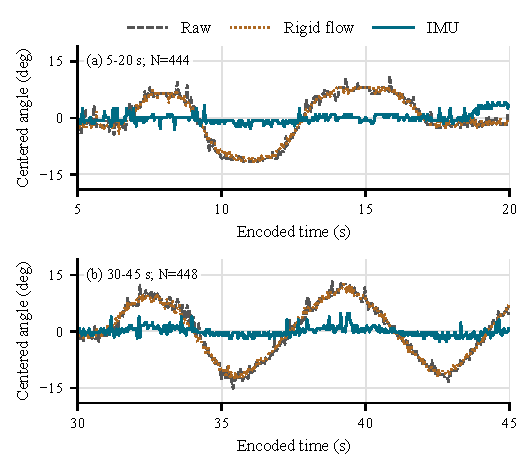
\includegraphics[width=\columnwidth]{figures/archived_marker_steadiness.pdf}
\caption{Physical-marker image orientation in two archived indoor intervals.
Each trace has its own common-support mean removed; gaps retain excluded
indices. The smaller variation of the IMU output is a saved-software result,
not a measurement of current FPGA leveling accuracy or absolute gravity.}
\label{fig:marker-traces}
\end{figure}

\subsection{Scope of the Inertial Diagnostics}
The archive also contains painted horizon and offline IMU-filter diagnostics.
A line derived from accelerometer attitude and the same
camera geometry used for correction tests model consistency, not an
independent physical horizon. The red-pixel extractor also selects scene
objects, demonstrably contaminating an indoor frame. The audit retains these
pixel statistics and support, without converting them through a nominal
pixels/degree constant into physical leveling errors.

The archived acquisition logs identify a RealSense D435i IMU, whereas the
current MCU uses the IIM46234 configuration in Section~\ref{sec:algorithm}.
The old filter comparison uses accelerometer angles from the same sensor as
its reference, includes centered five-sample averaging, and converts
correlation index shifts through a median sample interval despite irregular
timestamps. It cannot establish independent attitude accuracy, causal filter
delay, or the current system's latency. These diagnostics are retained for
reproduction, while hardware timing claims use the identified event boundaries
in Section~\ref{sec:hardware}.
